% This file was created with matplot2tikz v0.4.0.
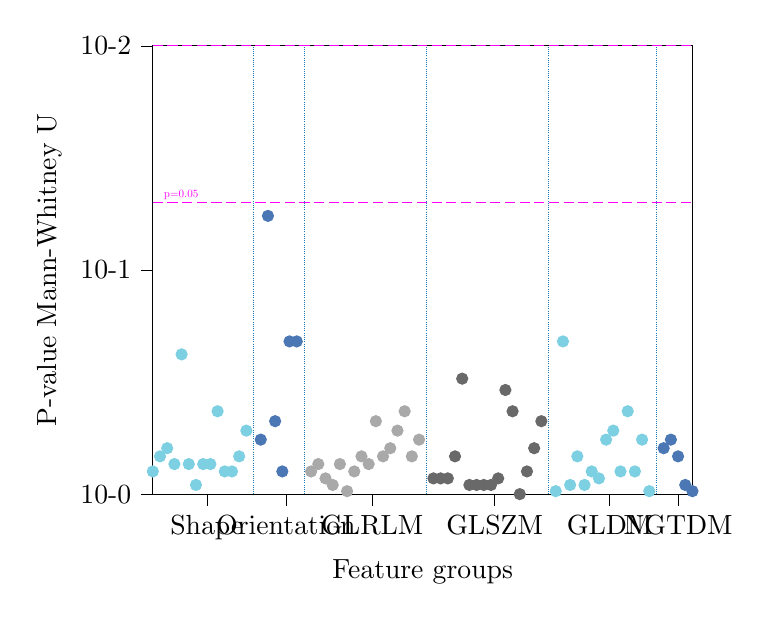
\begin{tikzpicture}

\definecolor{darkgray}{RGB}{169,169,169}
\definecolor{darkgray176}{RGB}{176,176,176}
\definecolor{dimgray}{RGB}{105,105,105}
\definecolor{fuchsia}{RGB}{255,0,255}
\definecolor{skyblue125207226}{RGB}{125,207,226}
\definecolor{steelblue31119180}{RGB}{31,119,180}
\definecolor{steelblue75120181}{RGB}{75,120,181}

\begin{axis}[
log basis y={10},
tick align=outside,
tick pos=left,
x grid style={darkgray176},
xlabel={Feature groups},
xmin=0, xmax=75,
xtick style={color=black},
xtick={7.5,18.5,30.5,47.5,63.5,73},
xticklabels={Shape,Orientation,GLRLM,GLSZM,GLDM,NGTDM},
y dir=reverse,
y grid style={darkgray176},
ylabel={P-value Mann-Whitney U},
ymin=0.01, ymax=1,
ymode=log,
ytick style={color=black},
ytick={1,0.1,0.01},
yticklabels={10-0,10-1,10-2}
]
\addplot [draw=skyblue125207226, fill=skyblue125207226, mark=*, only marks]
table{%
x  y
0 0.792077478764785
1 0.67843137254902
2 0.623878701278082
3 0.7344923394459
4 0.237977296181631
5 0.7344923394459
6 0.910105580693816
7 0.7344923394459
8 0.7344923394459
9 0.426863538937842
10 0.792077478764785
11 0.792077478764785
12 0.67843137254902
13 0.520806541239978
};
\addplot [draw=steelblue75120181, fill=steelblue75120181, mark=*, only marks]
table{%
x  y
15 0.571358259903152
16 0.0573787409700722
17 0.472668095578312
18 0.792077478764785
19 0.208287687544653
20 0.208287687544653
};
\addplot [draw=darkgray, fill=darkgray, mark=*, only marks]
table{%
x  y
22 0.792077478764785
23 0.7344923394459
24 0.850631102643487
25 0.910105580693816
26 0.7344923394459
27 0.969929348257522
28 0.792077478764785
29 0.67843137254902
30 0.7344923394459
31 0.472668095578312
32 0.67843137254902
33 0.623878701278082
34 0.520806541239978
35 0.426863538937842
36 0.67843137254902
37 0.571358259903152
};
\addplot [draw=dimgray, fill=dimgray, mark=*, only marks]
table{%
x  y
39 0.850631102643487
40 0.850631102643487
41 0.850631102643487
42 0.67843137254902
43 0.305390172263237
44 0.910105580693816
45 0.910105580693816
46 0.910105580693816
47 0.910105580693816
48 0.850631102643487
49 0.343145193299992
50 0.426863538937842
51 1
52 0.792077478764785
53 0.623878701278082
54 0.472668095578312
};
\addplot [draw=skyblue125207226, fill=skyblue125207226, mark=*, only marks]
table{%
x  y
56 0.969929348257522
57 0.208287687544653
58 0.910105580693816
59 0.67843137254902
60 0.910105580693816
61 0.792077478764785
62 0.850631102643487
63 0.571358259903152
64 0.520806541239978
65 0.792077478764785
66 0.426863538937842
67 0.792077478764785
68 0.571358259903152
69 0.969929348257522
};
\addplot [draw=steelblue75120181, fill=steelblue75120181, mark=*, only marks]
table{%
x  y
71 0.623878701278082
72 0.571358259903152
73 0.67843137254902
74 0.910105580693816
75 0.969929348257522
};
\path [draw=steelblue31119180, line width=0.12pt, dash pattern=on 0.3pt off 0.495pt]
(axis cs:14,1)
--(axis cs:14,0.01);

\path [draw=steelblue31119180, line width=0.12pt, dash pattern=on 0.3pt off 0.495pt]
(axis cs:21,1)
--(axis cs:21,0.01);

\path [draw=steelblue31119180, line width=0.12pt, dash pattern=on 0.3pt off 0.495pt]
(axis cs:38,1)
--(axis cs:38,0.01);

\path [draw=steelblue31119180, line width=0.12pt, dash pattern=on 0.3pt off 0.495pt]
(axis cs:55,1)
--(axis cs:55,0.01);

\path [draw=steelblue31119180, line width=0.12pt, dash pattern=on 0.3pt off 0.495pt]
(axis cs:70,1)
--(axis cs:70,0.01);

\path [draw=fuchsia, dash pattern=on 3.7pt off 1.6pt]
(axis cs:0,0.01)
--(axis cs:75,0.01);

\path [draw=fuchsia, dash pattern=on 3.7pt off 1.6pt]
(axis cs:0,0.05)
--(axis cs:75,0.05);

\draw (axis cs:1,0.0095) node[
  scale=0.4,
  anchor=base west,
  text=fuchsia,
  rotate=0.0
]{p=0.0007};
\draw (axis cs:1,0.0475) node[
  scale=0.4,
  anchor=base west,
  text=fuchsia,
  rotate=0.0
]{p=0.05};
\end{axis}

\end{tikzpicture}
